\documentclass[a5paper]{article}
\usepackage{graphicx}
\usepackage{hyperref}
\usepackage[final]{pdfpages}
\usepackage[parfill]{parskip}% don't indent new sections
\usepackage[utf8]{inputenc}
\usepackage{listings}
\usepackage{listings-golang}
\usepackage{color}
\usepackage[a4paper]{geometry}
\pagestyle{empty}

\lstset{frame=tb,
    frame=single,
    aboveskip=3mm,
    belowskip=3mm,
    showstringspaces=false,
    columns=flexible,
    basicstyle={\small\ttfamily},
    numbers=left,
    keywordstyle=\color{red},
    stringstyle=\color{blue},
    commentstyle=\color{dkgreen},
    breaklines=true,
    breakatwhitespace=true,
    tabsize=4,
    language=Golang
}

\title{Applied Algorithms}
\author{Emil Lynegaard}

\begin{document}
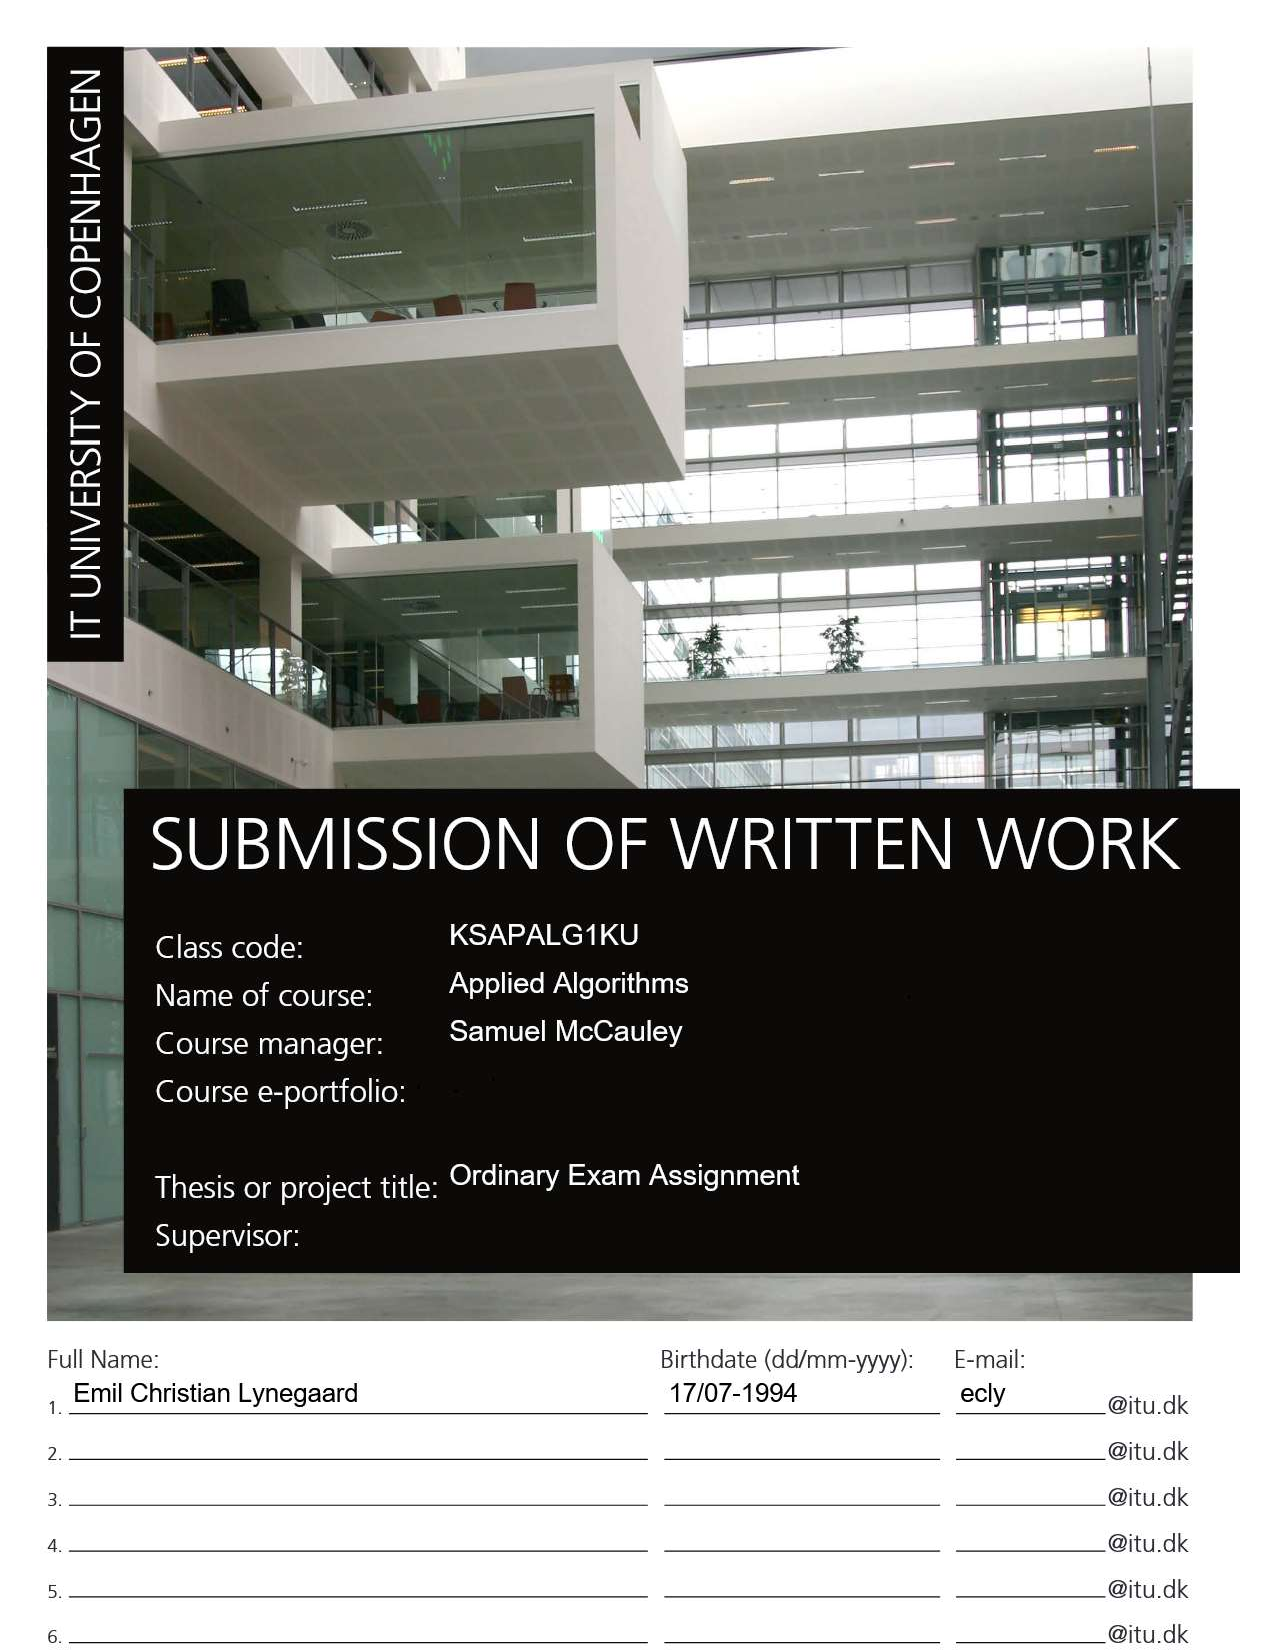
\includepdf[pages=1]{res/front_page.pdf}

\maketitle
\textit{I hereby declare that I have answered the exam questions myself without any outside help.}\\
\newpage

\newpage
\tableofcontents
\newpage

\section{Independent Set in Interval Graphs}
\subsection{}
Implementation is seen in file \texttt{independent\_set.go}.

\subsection{}
\textbf{(a)} 
The implementation has a running time of  $O(n^2)$.

\textbf{(b)}
If we only use $A_r$ and keep track of the right endpoint ($r$) of the element most recently added to the independent set.
Now we can remove the head of $A_r$ one by one, discarding elements with left endpoints ($l$) where $l \leq r$, and adding
elements with $l > r$. This way we only have to run through $A_r$ once, giving us $O(n)$ after sorting.

\textbf{(c)}
Since both lists are sorted in increasing order, albeit on different properties, by searching from the start of the list
we have a very good chance of finding it quickly. In the example on Figure 1 from the assignment, we will for example
find the first interval [-2, -1] as the second element when we try to remove it from the list sorted by interval start.

\textbf{(d)}
We use $l_2 \leq r$ for the inner loop since we want to discard all intervals that start before the end of the interval
that we have just added to the independent set.

\textbf{(e)}
If $A_r$ and $A_l$ were priority queues, other than the regular insert and pull, we would need a \texttt{remove(elem)} method to remove
a specific element somewhere in the queue.

\begin{lstlisting}
package main

import "fmt"

func main() {
    fmt.Println("Hello World!")
}
\end{lstlisting}

% \begin{figure}[!ht]
%     \centering
%     \noindent\includegraphics[scale=0.5]{res/}
%     \caption{}
%     \label{fig:}
% \end{figure}

\section{Appendix}
%\subsection{SecComSys.java}\label{sec:akka}
%\lstinputlisting{../src/Erlang/SecComSys.java}
\end{document}
